% !TEX encoding = IsoLatin2  % notwendige Zeile für Mac-Benutzer (muss als Kommentar stehen); Windows-Benutzer können die Zeile löschen.

% LaTeX-Vorlage Version 3.1,  Juli 2011
% erstellt von Dr. Andreas Drauschke (andreas.drauschke@technikum-wien.at) und Dr. Susanne Teschl (susanne.teschl@technikum-wien.at)
% geringfügig adaptiert von Harald Stockinger (harald.stockinger@technikum-wien.at)

 
\documentclass[a4paper,bibtotoc,oneside]{scrbook} 
% Für kurze Arbeiten wäre auch die Dokumentklasse "scrartcl" ausreichend. In diesem Fall ist "section" die höchste Ebene ("chapter" gibt es dann nicht).
% \documentclass[a4paper,bibtotoc,oneside]{scrartcl}

%\usepackage{cclicenses}

% javascript highlightning support
\usepackage{listings}
\usepackage{color}
\definecolor{lightgray}{rgb}{.9,.9,.9}
\definecolor{darkgray}{rgb}{.4,.4,.4}
\definecolor{purple}{rgb}{0.65, 0.12, 0.82}

\lstdefinelanguage{JavaScript}{
  keywords={typeof, new, true, false, catch, function, return, null, catch, switch, var, if, in, while, do, else, case, break},
  keywordstyle=\color{blue}\bfseries,
  ndkeywords={class, export, boolean, throw, implements, import, this},
  ndkeywordstyle=\color{darkgray}\bfseries,
  identifierstyle=\color{black},
  sensitive=false,
  comment=[l]{//},
  morecomment=[s]{/*}{*/},
  commentstyle=\color{purple}\ttfamily,
  stringstyle=\color{red}\ttfamily,
  morestring=[b]',
  morestring=[b]"
}
\lstset{
   language=JavaScript,
   backgroundcolor=\color{lightgray},
   extendedchars=true,
   basicstyle=\footnotesize\ttfamily,
   showstringspaces=false,
   showspaces=false,
   numbers=left,
   numberstyle=\footnotesize,
   numbersep=9pt,
   tabsize=2,
   breaklines=true,
   showtabs=false,
   captionpos=b
}

% verlinkte Querverweise im pdf
\usepackage{hyperref}

% deutsche Anpassungen
\usepackage[utf8]{inputenc}
\usepackage[T1]{fontenc}
\usepackage[ngerman]{babel}


% mathematische Symbole
\usepackage{amsmath,amssymb,amsfonts,amstext}

% Kopfzeilen frei gestaltbar
\usepackage{fancyhdr}
\lfoot[\fancyplain{}{}]{\fancyplain{}{}}
\rfoot[\fancyplain{}{}]{\fancyplain{}{}}
\cfoot[\fancyplain{}{\footnotesize\thepage}]{\fancyplain{}{\footnotesize\thepage}}
\lhead[\fancyplain{}{\footnotesize\nouppercase\leftmark}]{\fancyplain{}{}}
\chead{}
\rhead[\fancyplain{}{}]{\fancyplain{}{\footnotesize\nouppercase\sc\leftmark}} 

% Farben im Dokument möglich
\usepackage{color}

% Schriftart Helvetica
\usepackage{helvet}
\renewcommand{\familydefault}{cmss} 

% Graphiken einbinden: hier für pdflatex
\usepackage[pdftex]{graphicx}

\usepackage{array}

% Höhe und Breite des Textkörpers etwas grösser definieren
\setlength{\textheight}{225mm}
\setlength{\textwidth}{1.05\textwidth}

% weniger Warnungen wegen überfüllter Boxen
\tolerance = 9999
\sloppy

% Anpassung einiger überschriften 
\renewcommand\figurename{Abbildung}
\renewcommand\tablename{Tabelle}

\begin{document}

% Kopf- und Fusszeilen initiieren
\pagestyle{fancy}
\pagenumbering{Alph}

% Deckblatt:
\thispagestyle{empty}
\begin{picture}(0,0)
\color{white}\sffamily
\put(-101,-749){
\includegraphics[width=1.002\paperwidth, height=\paperheight]{BM_2011.pdf}}
\put(220,-670){
\includegraphics[width=0.5\textwidth]{FHTW_Logo_4c.pdf}}
\put(-30, -20){\bfseries\huge BACHELORARBEIT}
% Titel des Studienganges einfügen:
\put(-30,-50){\Large im Studiengang Bachelor Informatik}
% Titel der Arbeit einfügen:
% Die Minipage wird gesetzt, damit auch mehrzeilige Titel möglich werden.
\put(-32,-150){
\begin{minipage}{14cm}
\bfseries\huge Software-Test von Web-Applikationen
\end{minipage}
}
% Name der Autorin/des Autors eingeben:
\put(-30,-250){\large Ausgeführt von: Bernhard Posselt}
% Personenkennzeichen der Autorin/des Autors eingeben:
\put(-30,-270){\large Personenkennzeichen: 1010257029}
% Name der Begutachterin/des Begutachters eingeben:
\put(-30,-310){\large Begutachter: MSc Benedikt Salzbrunn}
\put(-30,-350){\large Wien, \today} % das Datum des letzten Kompilierens wird automatisch eingesetzt
\color{black}
\end{picture}

\newpage


\section*{Eidesstattliche Erklärung}\thispagestyle{empty}
\glqq Ich erkläre hiermit an Eides statt, dass ich die vorliegende Arbeit selbständig angefertigt habe. 
Die aus fremden Quellen direkt oder indirekt übernommenen Gedanken sind als solche kenntlich gemacht. 
Die Arbeit wurde bisher weder in gleicher noch in ähnlicher Form einer anderen Prüfungsbehörde vorgelegt
und auch noch nicht veröffentlicht. Ich versichere, dass die abgegebene Version jener im Uploadtool entspricht.\grqq\\[5\baselineskip]
\rule{5cm}{0.2pt}\hfill\rule{5cm}{0.2pt}\\
\phantom{Datum }Ort, Datum\hfill Unterschrift\hspace{15mm}

\newpage


\section*{Kurzfassung}\thispagestyle{empty}
Die Durchführung und Erstellung von automatisierten Tests für Web-Applikationen unterscheidet sich von klassischen Applikationen. Aufgrund der komplexeren Infrastruktur und Modularisierung werden zusätzliche Testfälle und Strategien benötigt um Web-Applikationen ausreichend abzudecken und eine fortwährende Qualität zu gewährleisten. Diese Arbeit soll Möglichkeiten für den Test von Web-Applikationen anhand eines Projektes aufzeigen und Anpassungen und Anwendung der vier Testformen des V-Modells: Unit Test, Integration Test, System Test und Acceptance Test. 

\vfill
\paragraph*{Schlagwörter:} Webapplikationen, automatisierte Tests, Webtest


\newpage

\section*{Abstract}\thispagestyle{empty}
Creation and execution of automatic web application tests is different from tests of classic applications. A more complex infrastructure and modularisation require additional testcases and strategies to guarantee a good enough test coverage which in return ensures constant quality. This thesis highlights various possibilities to test web applications based on a real world project and shows how to use and adjust the V-Model's four test methods: Unit Test, Integration Test, System Test and Acceptance Test.

\vfill
\paragraph*{Keywords:} web applications, automatic tests, webtest
\newpage

%\section*{Danksagung}
%\thispagestyle{empty}
%Text Text Text Text Text Text Text Text Text Text Text Text Text Text Text Text
%\newpage

\tableofcontents\thispagestyle{empty}
\newpage

\pagenumbering{arabic}
\setcounter{page}{1}

% Falls die Kapitelüberschriften zu lang für die Kopfzeile oder das Inhaltsverzeichnis sind, so erzielt man
% dort Kurzformen der Kapitelbezeichnungen mittels:
% \chapter[Kurzform]{Lange überschrift}
\chapter{Einführung}
Der Markt für elektronische Geräte hat in den letzten Jahren ein rasantes Wachstum erlebt, vor allem im Bereich der mobilen Geräte. Im Jahr 2011 wurden erstmals mehr mobile Geräte verkauft als PCs \ref{Abb1}.
Durch dieses Wachstum dehnt sich auch der Markt für Software-Applikationen auch auf mobile Geräte aus, welche zum Großteil andere Betriebssysteme und Applikations-Frameworks verwenden als traditionelle Computer \ref{Abb2}. Viele dieser Plattformen erfordern das Erlernen von unterschiedlichen Programmiersprachen, Frameworks und Betriebssystemen \cite{android}\cite{ios}. Will ein/eine Software-EntwicklerIn eine Applikation plattformübergreifend anbieten, erfordert dies daher einen höheren Zeit- und Kostenaufwand.

\begin{figure}[h!]
\centering
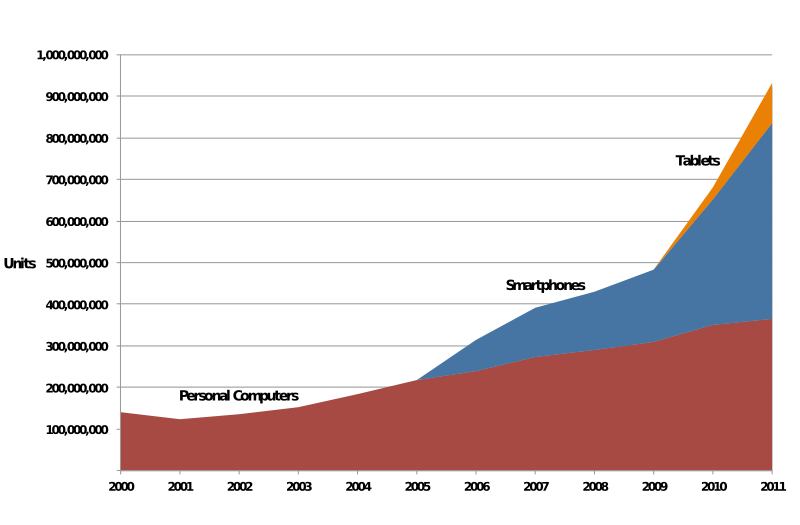
\includegraphics[width=150mm]{img/globaldevicesales.png}
\caption[Entwicklung der PC und Mobilgerätverkäufe]{Entwicklung der PC und Mobilgerätverkäufe \cite{devicesales}[S. 6]}\label{Abb1}
\end{figure}

Da viele dieser Mobilgeräte über einen Web-Browser verfügen, wird das Web als Applikations-Plattform immer attraktiver. Zudem erlauben Frameworks wie PhoneGap \cite{phonegap} dem/der EntwicklerIn eine plattformübergreifende Mobil-Applikation auf Basis von Web-Technologien zu erstellen, welche sich nahtlos in das System integrieren. 

\begin{figure}[h!]
\centering
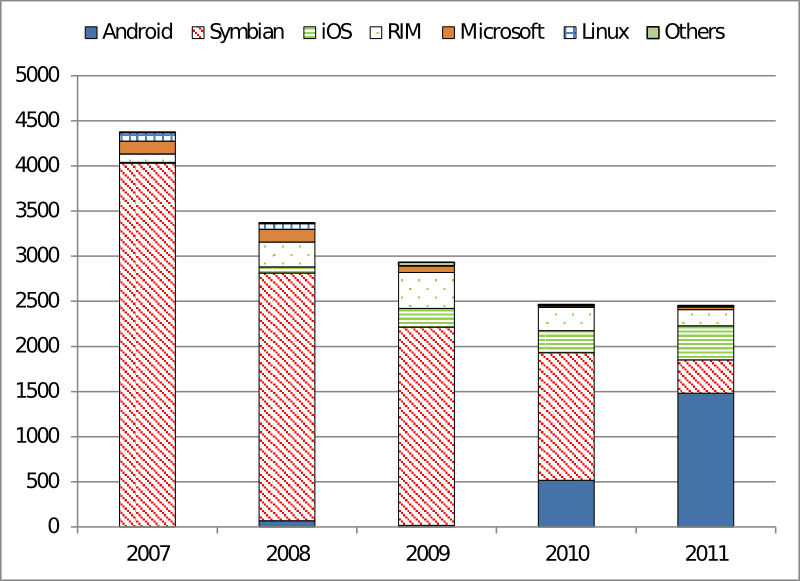
\includegraphics[width=100mm]{img/operatingsystems.png}
\caption[Marktanteil mobiler Betriebssysteme]{Marktanteil mobiler Betriebssysteme \cite{smartphone}[S. 22]}\label{Abb2}
\end{figure}


\section{Problemstellung}
Aufgrund der Vielfalt an unterschiedlichen Web-Browsern erhöht sich jedoch auch der Testaufwand der Applikation. Die Browser implementieren die vom W3C vorgeschlagenen Standards ab und zu anders und in unterschiedlicher Geschwindigkeit. Nicht selten kommt es vor, dass gewisse Funktionen nur in einer eingeschränkten Auswahl von Web-Browsern voll funktionsfähig sind und zusätzliche Anpassungen erfordern. \cite{caniuse}

Ein weiteres Problem ist das verhaltene Upgradeverhalten der NutzerInnen. Im Falle des Internet Explorers 7 dauerte es mehr als 19 Monate bis rund die Hälfte der NutzerInnen auf die neue Version umgestiegen sind. \cite{insecure}[S. 3]


\section{Lösungsansatz}
Um eine konstante Qualität der Web-Applikation auf allen Plattformen zu gewährleisten, muss das bisherige Testssystem angepasst werden, um der höheren Komplexität von Web-Applikationen gerecht zu werden. 

Diese Bachelorarbeit soll die zusätzlichen Herausforderungen beim Testen von Web-Applikationen aufzeigen. Des Weiteren soll sie einen Überblick über mögliche Anwendungen und Anpassungen der vier häufigsten Testarten - den Unit Tests, Integration Tests, System Tests und Acceptance Tests - im Bereich der Web-Applikationen geben.

Dazu wird anhand eines Projektes eine Test-Strategie erarbeitet und Beispiele für Tests gegeben.


\section{Aufbau}
Kapitel 2 behandelt den Sinn und die Grenzen des Software-Tests und wie er sich in den Entwicklungsprozess einbinden lässt.

In Kapitel 3 wird auf die Unterschiede zwischen klassischen Applikationen und Web-Applikationen eingegangen. Dadurch sollen zusätzliche Probleme, die sich durch das Applikations-Modell ergeben, aufgezeigt werden.

Die Planung und der Ablauf des Testprozesses durch die Verwendung eines Testplanes Kapitel 4 beschrieben.

Kapitel 5 beschäftigt sich näher mit dem praktischen Einsatz von Unit Tests, welche serverseitigen und clientseitigen Quellcode abdecken.

Das Thema des Integration Tests wird in Kaptitel 6 behandelt und zeigt dessen Einsatzzweck bei Web-Applikationen.

Kaptitel 7 behandelt den Systemtest und dem Test der verschiedenen Plattformen.

Kapitel 8 beschäftigt sich mit dem Thema des Acceptance Tests und wie dieser bei Web-Applikationen umgesetzt werden kann.

\chapter{Warum testen}
Keine Applikation ist fehlerfrei\cite{empiric_invest}[S. 9]. Diese Fehler  führen nicht nur zu unzufriedenen Kunden, sondern auch zu hohen Kosten: \glqq Im Jahr 2000 wurde in den USA ein Schaden durch Softwarefehler in der Auto- und Flugzeugindustrie von 1,8 Milliarden US-Dollar errechnet. Dies entspricht ca. 16 \% des Softwareumsatzes.\grqq\cite{betrieb}[S. 15]

Die Fehler-Rate wird auf ungefähr 3 pro 1.000 Zeilen geschätzt, was bei einer aufwendigeren Applikation mit 100 Millionen Zeilen Quellcode eine durchschnittliche Anzahl von 300.000 Fehlern ergibt \cite{eval_regression}[S. 10]. 

Je früher diese Fehler entdeckt werden, desto kostengünstiger können diese beseitigt werden \cite{betrieb}[S. 17]. Daher ist es wichtig, möglichst früh mit dem Testen zu beginnen und den Software-Entwicklungsprozess dementsprechend anzupassen \cite{betrieb}[S. 16]. 

\section{Verschiedene Testarten}
Eines der bekanntesten Testmodelle stellt das V-Modell dar \ref{Abb3}. Dieses unterteilt die verschiedenen Testbereiche in vier Kategorien: 

\begin{itemize}
	\item Unit Test
	\item Integration Test
	\item System Test
	\item Acceptance Test
\end{itemize}

\begin{figure}[h!]
\centering
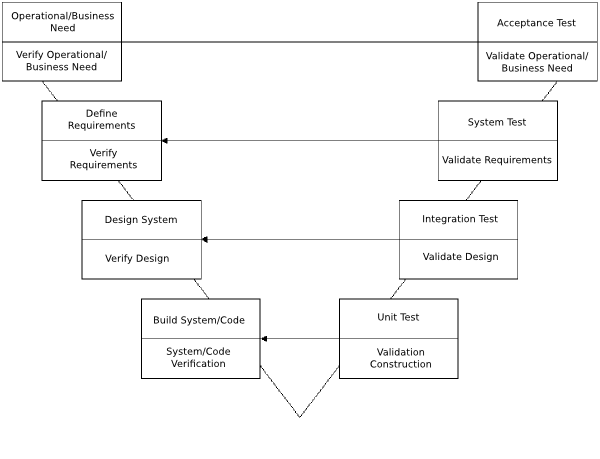
\includegraphics[width=120mm]{img/vmodel.png}
\caption[Schematische Darstellung des V-Modells]{Schematische Darstellung des V-Modells \cite{vmodel}[S. 3]}\label{Abb3}
\end{figure}

Im linken Berech befinden sich die jeweiligen Schritte zur Erstellung der Applikation. Diesen gegenübergestellt werden die jeweiligen Testarten. Damit soll veranschaulicht werden, dass der Testprozess kein in sich geschlossener Abschnitt ist, sondern sich stark in den Entwicklungsprozess integriert \cite{betrieb}[S. 23]

Diese vier verschiedenen Testarten lassen sich unterschiedlich gut manuell und automatisch testen.

\section{Manuelle Tests}
Manuelle Tests eignen sich vor allem im Bereich des System-Tests und Acceptance-Tests, da sich diese Bereiche oft schwer komplett automatisch testen lassen. Diese Tests umfassen unter anderem die Kontrolle der Übersetzungen und der Dokumentation. Auch die dazu gehörenden Usability-Tests lassen sich schwer bis überhaupt nicht automatisieren und erfordern zum Großteil manuelle Tests. \cite{test_large_systems}[S. 61]


\section{Automatisierten Tests}
Da die vorhandenen Tests durch die Einbindung in den Entwicklungsprozess öfters durchgeführt werden müssen, kann sich durch das manuelle Testen der immer gleichen Tests schnell eine gewisse Eintönigkeit einstellen. Das wiederum kann unter anderem dazu führen, dass Tester bestimmte Tests nicht korrekt oder ineffizient ausführen. 

Dieses Problem kann durch eine Automatisierung des Testprozesses gelöst werden. Die Automatisierung erlaubt zudem bei zukünftigen Testdurchläufen eine Reduzierung auf ein Minimum des ursprünglichen Zeitaufwandes. Daher sollte versucht werden, möglichst viele dieser Tests zu automatisieren. \cite{test_auto}[S. 22-23]. 
d
Automatisierte Tests eignen sich besonders für Bereiche, die gut automatisiert getestet werden können. Dies betrifft vor allem die Unit-Tests und Integration-Tests, jedoch können auch System- und Acceptance Tests zum Teil automatisiert getestet werden, beispielsweise kann der Installationsprozess automatisch geprüft werden. Zudem kann es vorkommen, dass nicht genügend geschultes Personal für automatische Tests vorhanden ist. \cite{eval_automat_webapp_test}[S. 37]

Auch können automatisierte Tests rund um die Uhr ausgeführt werden, was eine effizientere Nutzung der Zeit garantiert.

\section{Testen im Projektzyklus}
Tests können jedoch nicht nur dazu verwendet werden, um Fehler in der Applikation zu finden, sondern auch um einen Überblick über den derzeitigen Stand der Implementation zu gewinnen: Sie geben dem/der EntwicklerIn und ProjektmanagerIn ein direktes Feedback über bereits korrekt implementierte Teile der Software-Spezifikation. Auch Milestones können durch Tests definiert werden. \cite{test_auto}[S. 2]

Zudem ist eine Abschätzung riskanter Bereiche möglich, die durch eine erhöhten Testbedarf bestimmter Bereiche offensichtlich wird. \cite{testing_apps_on_web}[S. 34]


\section{Grenzen von Software-Tests}
Das Vorhandensein von Tests kann niemals eine komplett fehlerfreie Software garantieren, nur eine Abwesenheit von bestimmten Fehlern kann garantiert werden, nämlich jenen, die explizit mit Tests abgedeckt werden \cite{eval_regression}[S. 12]. Dies resultiert unter anderem daraus, dass die Anforderungen an die Software oft nicht komplett spezifiziert oder ungenau sind und die Komplexität der Applikation im Laufe der Entwicklung stark ansteigt. Zusätzlich können die Testfälle durch die vielen möglichen Eingaben lediglich einen kleinen Bereich der Funktionsweise abdecken \cite{software_qual}[S. 243].

Es ist jedoch nicht erstrebenswert, die ganze Applikation mit Tests abzudecken, da dies zu zu hohen Entwicklungskosten führen kann. Idealerweise werden daher nur jene kritischen Fälle mit Tests abgedeckt, deren Fehlerkosten die Kosten für die Erstellung der Tests übertreffen. \cite{eval_regression}[S. 12]

Die implementierten Testfälle müssen auch regelmäßig gewartet und aktualisiert werden, um ihre Effektivität zu gewährleisten, denn diese nimmt auf Dauer ab. Es ensteht eine sogenannte \glqq Testresistenz\grqq\cite{eval_regression}[S. 12], die daraus resultiert, dass die bestehenden Tests nur bekannte Fehlerfälle abdecken und neue mögliche Fehlerfälle nicht berücksichtigen. \cite{eval_regression}[S. 12-13]

\chapter{Testplan}

Mit dem Erstellen des Projektplanes sollte gleichzeitig auch ein Testplan erstellt werden \cite{eval_automat_webapp_test}[S. 24]. Dieser erlaubt, den Testprozess näher zu spezifizieren und somit den erforderlichen Aufwand besser abschätzen zu können \cite{test_large_systems}[S. 18] und den Testprozess eventuell an ein externes Team auszulagern. Zusätzlich kann der Plan auch dazu verwendet werden, die Abnahmekriterien exakt zu definieren, um das Projektrisiko zu verringern. \cite{eval_automat_webapp_test}[S. 26]

\section{Inhalt}
Im Testplan werden unter anderem folgende Punkte behandelt \cite{test_auto}[S. 3]:

\begin{itemize}
	\item Was wird getestet? Welche Bereiche besitzen eine höhere Priorität als andere?
	\item Wo wird getestet? Mit welchen Konfigurationen, Soft- und Hardware Plattformen respektive Versionen werden getestet?
	\item Wie wird getestet? mit welchen Tools wird getestet?
	\item Wer testet?
	\item Wie lange wird getestet? Bis wann muss ein Test erfolgreich absolviert werden?
	\item Was wird nicht getestet?
\end{itemize}


\section{Ablauf}
Da die Entwicklung der Applikation meistens mit einem hohen Zeitdruck verbunden ist\cite{software_qual}[S. 244] und der Testprozess zudem teuer ist \cite{eval_regression}[S. 24], ist es wichtig, die Testfälle heraus zu arbeiten, zu priorisieren und effektiv zu verteilen. Des Weiteren werden Endkriterien für die Tests veranschlagt und die optimale Teststrategie gewählt.

Danach folgt die Überprüfung des Testplans. Hier wird überprüft ob die einzelnen Testfälle genau genug beschrieben worden sind, um daraus die jeweiligen Testfälle erstellen zu können und ob die Teststrategien angemessen sind. Da die gesamten Anforderungen an die Applikation oft erst im Laufe des Projektes klar werden, muss der Testplan regelmäßig auf Korrektheit und Angemessenheit überprüft und dementsprechend angepasst werden. \cite{eval_regression}[S. 25] 

Ist der Testplan soweit fertig, kann ein Zeitplan für die einzelnen Testfälle festgelegt werden. In weiterer Folge werden die einzelnen Tests an die TesterInnen vergeben, welche dann mit der Erstellung der dazu gehörigen Testfälle beginnen können.

Um den Ablauf der Tests zu beschleunigen, sollten unnötige Testdurchläufe vermieden werden. Dies wird mit der Erstellung eines Smoke-Tests erreicht, dessen Aufgabe es ist, essentielle Testszenarien durchzutesten. Schlagen diese fehl, sind weitere Testdurchläufe nicht notwendig und der Testdurchlauf kann abgebrochen werden. 

Nach dem Ausführen der Tests wird ein Bericht erstellt. Je nach Ausgang der Tests muss der Testplan angepasst werden. Verliefen alle Tests positiv, kann das Testen für die jeweilige Phase beendet werden. \cite{eval_regression}[S. 26]


\section{Vorteile eines Testplans}

Aufgrund der Dokumentation der Testfälle, ergeben sich zusätzlich folgende Vorteile:

\begin{itemize}
	\item Fehlende Testfälle können schnell erkannt werden \cite{test_large_systems}[S. 18]
	\item Redundante Testfälle werden identifziert, Testfälle können zusammegelegt werden um Zeit zu sparen \cite{testing_apps_on_web}[S. 34]
	\item Verschiedene Testbereiche können an mehrere Personen mit unterschiedlichen Fachkenntnissen verteilt werden um Personalengpässe zu vermeiden \cite{test_large_systems}[S. 19]
	\item Ineffiziente Test-Tools und Test-Strategien können erkannt und verbessert werden \cite{eval_regression}[S. 25]
	\item Geschäftskritische Bereiche und solche mit einer erhöhten  Fehleranfälligkeit werden sichtbarer \cite{testing_apps_on_web}[S. 34]. Dies ist vor allem wichtig, da Fehler ungleich verteilt sind und in bestimmten Bereichen häufiger vorkommen als in anderen \cite{eval_regression}[S. 12]
	\item Sinnlose Testfälle und Testbereiche können aussortiert werden 
	\item Abhängigkeiten der Testfälle untereinander und der Implementation werden transparent und erlauben schnell auf Änderungen zu reagieren\cite{test_auto}[S. 4]
\end{itemize}


\chapter{Unterschiede zu klassischer Software}
Eine Web-Applikationen unterscheidet sich an mehreren Stellen von einer klassichen Applikation, was das Testen und das Auffinden von Fehlern zusätzlich erschwert. Die Hauptunterschiede sind:

\begin{itemize}
	\item Modularer Aufbau
	\item Plattformunabhängigkeit
	\item Session Modell
\end{itemize}


\section{Modularer Aufbau}

Im Gegensatz zu klassischen Desktop- oder Mobil-Applikationen bestehen Web-Applikationen wegen ihrer Client-Server-Architektur immer aus mehreren Modulen \ref{Abb4}, die meist über ein Netzwerk miteinander verbunden sind.

Durch diesen modularen Aufbau ist es besonders schwer einen Fehler zu lokalisieren. Ein Fehler kann z.B. durch einen Fehler im Quellcode des Applikations-Servers oder durch ein Netzwerkproblem entstanden sein. \cite{testing_apps_on_web}[Foreword]

\begin{figure}[h!]
\centering
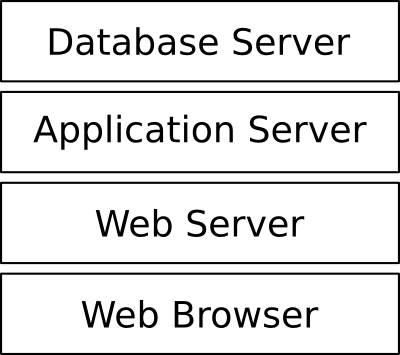
\includegraphics[width=50mm]{img/webstack.png}
\caption[Schematischer Aufbau einer Web-Applikation]{Schematischer Aufbau einer Web-Applikation}\label{Abb4}
\end{figure}

\section{Unterstützung mehrerer Plattformen}
Web-Applikationen laufen auf einer Vielzahl verschiedener Plattformen, Server- und Clientseitig. Dies ermöglicht dem/der EntwicklerIn Zeit und Aufwand zu sparen, befreit ihn/sie jedoch nicht von der Aufgabe, sicher zu stellen, dass die Applikation auf möglichst vielen Plattformen korrekt ausgeführt wird.

Während auf der Serverseite die jeweilig zu verwendenden Plattformen noch vom/von der BetreiberIn festlegbar sind, sprich welches Betriebssystem und welche Datenbank eingesetzt wird, ist dies auf der Clientseite schon nicht mehr möglich. 

Die BesucherInnen der Webseite verwenden unterschiedliche Web-Browser auf verschiedenen Betriebssystemen, welche beide in unterschiedlichen Versionen vorliegen können. Auch können unterschiedliche Plugins und Fonts in unterschiedlichen Versionen installiert sein \cite{testing_apps_on_web}[Foreword]. Dies erhöht den Testaufwand, da bestimmte Funktionen nicht vorhanden sein bzw. anders funktionieren können \cite{caniuse}.

Zudem verlagert sich auch immer mehr Applikations-Logik von der Server- auf die Clientseite\cite{testing_apps_on_web}[S. 13], was dieses Problem noch verstärkt. Außerdem stellt diese Verschiebung den/die EntwicklerIn vor noch größere Herausforderungen.

Web-Browser setzen stark auf asynchrone und eventbasierte Programmierung. Dies erschwehrt nicht nur die Erstellung von Testfällen sondern erhöht auch die möglichen Kombinationen, in der die Events eintreten können. Die Möglichkeit, dass durch eine Aktion, z.B. ein Mausklick auf einen Link, mehrere Events ausgelöst werden können erhöht die Komplexität noch mehr. \cite{testing_apps_on_web}[S. 18]

\section{Session Modell}
Eine weitere Herausforderung stellt das Session Modell von Web-Applikationen dar: viele Web-Applikationen verwenden nur eine Session pro NutzerIn, erlauben aber mehrere gleichzeitige Logins. Werden mehrere Instanzen der Applikation gestartet - z.B. loggt sich der/die NutzerIn auf dem Mobiltelefon und dem Laptop auf der Webseite ein - kann dies zu Synchronisationsproblemen zwischen den einzelnen Instanzen führen: Wird in einer Instanz ein Eintrag gelöscht, kann dieser durch eine fehlerhafte Synchronisation in einer andere Instanz immer noch existieren und in weiterer Folge zu Fehlern führen. \cite{testing_apps_on_web}[S. 20]

Diese Vielfalt an verschiedenen möglichen Konfigurationen und Herausforderungen erfordert eine neue Herangehensweise an das Thema Software-Test: Die bestehenden Techniken sind \glqq zwar auch notwendig, aber nicht ausreichend, um die Qualität der Applikation sicherzustellen\grqq\ \cite{eval_automat_webapp_test}[S. 18]


\chapter{Projektumfeld}

% TODO: warum spannend, aufbau des projektes

\chapter{Unit Test}
Unit Tests werden verwendet, um Klassen, Module oder einzelne Komponenten zu testen. Sie sind Whitebox Tests, sprich die Implementationsdetails sind bekannt\cite{betrieb}[S. 26], und werden üblicherweise vom Programmierer selbst erstellt. 

Zu den Vorteilen von Unit Tests zählen:

\begin{itemize}
	\item Gute Paralellisierbarkeit
	\item Sehr schnell ausführbar
	\item Früh einsetzbar
	\item Erlaubt die Aufteilung in kleine Teilprobleme
	\item Zeigt schwer zu verwendende Interfaces auf
\end{itemize}

Viele dieser Vorteile resultieren daraus, dass Unit Tests nicht auf andere Komponenten angewiesen sind, da diese üblicherweise durch Mocks bereitgestellt werden. 

Nur Unit Tests alleine reichen jedoch nicht aus, um das Projekt komplett abzudecken, da sie keine Kommunikation zwischen den einzelnen Komponenten testen. Auch Tests für verschiedene Datenbanken können dadurch nicht abgedeckt werden. \cite{test_large_systems}[S. 52]\cite{betrieb}[S. 28]

\section{Serverseitige Unit Tests}
Serverseitige Unit Tests unterscheiden sich nicht nur anhand des eingesetzten Test-Frameworks, sondern auch anhand der gewählten Programmiersprache. 

%todo

\section{Clientseitige Unit Tests}
Im Gegensatz zum serverseitigen Code gibt es auf der Clientseite nur eine mögliche Programmiersprache, um Logik plattformübergreifend zu implementieren: \emph{JavaScript}. Für JavaScript gibt es mehrere Test-Frameworks, darunter Jasmine \cite{jasmine}, QUnit \cite{qunit} und Mocha \cite{mocha}.
In dieser Arbeit wird für die Implementation der clienseitigen Unit Tests Jasmine eingesetzt.

\subsection{Häufige Probleme bei clientseitigem Code}
Das Web ist noch recht jung und wurde bis zur Entstehung des Begriffes \emph{Web 2.0} oft nur für einfache Webseiten verwendet. Die erste Web 2.0 Konferenz wurde im Oktober 2004 abgehalten mit dem Ziel, das Web als Plattform zu stärken. \cite{web2}[S. 19]

Viele der Probleme beim Testen von clientseitigem Code entstehen daher dadurch, dass die EntwicklerInnen noch nicht so sehr mit der Technologie vertraut sind und anfälliger für Architektur-Fehler sind.

\subsubsection{Fehlende Trennung von Logik und Präsentation}
Die mit Abstand am beliebtesten Clientseitige JavaScript Library ist jQuery. Im Jahr 2011 verwendeten laut Alexa 45\% der Top 100.000 Webseiten eine JavaScript Library. Von diesen 45\% entfielen 63\% auf jQuery. \cite{jquery}[S. 107-108]

jQuery ist sehr einfach zu verwenden \cite{jquery}[S. 110], verleitet jedoch aufgrund der Funktionsweise dazu, Präsentation und Logik stark miteinander zu verweben. Dies liegt unter anderem daran, dass jQuery als ersten Parameter einen Selektor erwartet. Dieser Selektor funktioniert ähnlich wie ein CSS Selector und selektiert bestimmte Element im DOM. \cite{jquery_selectors}

Folgender Code soll dieses Problem verdeutlichen: Der angeführte Code führt einen AJAX Request aus und gibt abhängig von der zurückgegebenen Datenstruktur einen unterschiedlichen Text aus:

\lstinputlisting[language=Html]{src/jquery.html}
\lstinputlisting[language=JavaScript]{src/jquery.js}

Durch das verwenden des Selektors \emph{\#field .info div} ist der JavaScript Code nun abhänig von der HTML Struktur der Webseite. Verändert ein Designer  die Struktur des HTML-Codes, beispielsweise um die Ausgabe an einen anderen Ort zu verschieben, besteht die Gefahr, dass der Selektor nicht mehr die gewollten Elemente selektiert und damit der JavaScript-Code nicht mehr funktioniert.

\subsubsection{Verwendung von Globalen Objekten und Variablen}
In JavaScript macht es einfach, globale Variablen zu verwenden. Es unterstützt nicht nur implizite \emph{Globals}\cite{js_patterns}[S. 11], sondern regelt den Zugriff auf das DOM über das globale \emph{window} Objekt\cite{js_patterns}[S. 13].

Dadurch werden ProgrammiererInnen absichtlich oder unabsichtlich dazu verleitet, globale Variablen und Objekte zu benutzen. Das wiederum erschwert die die Testbarkeit, da eine implizite Abhängigkeit von diese globalen Variablen und Objekten ensteht, die für den Tester nicht sofort offensichtlich ist. Auch wird es schwieriger, den Code in Isolation zu testen.

\subsection{Lösungsansatz}
Die vorher aufgezeigten Probleme können mit durch folgende Techniken gelöst werden:

\begin{itemize}
	\item Trennung der Logik und Präsentation durch Templates
	\item Vermeidung von globalen Objekten und Variablen
	\item Verwendung der Software-Patterns Dependency Injection und Inversion of Control, um Abhängigkeiten von Objekten und Funktionen offensichtlich zu machen
\end{itemize}

Um dies zu erreichen wird das JavaScript Framework \emph{AngularJS}\cite{angular} eingesetzt.

\subsubsection{Trennung von Logik und Präsentation}
AngularJS verfügt über eine eigene Template-Sprache, die durch selbst definierte HTML-Attribute umgesetzt ist. Dies erlaubt eine tiefe Integration in den vorhandenen HTML Code.

Mit AngularJS würde das vorige jQuery Beispiel in etwa so aussehen:

\lstinputlisting[language=Html]{src/angular.html}
\lstinputlisting[language=JavaScript]{src/angular.js}

Das \emph{Scope} dient als Schnittstelle zwischen der Logik und der Präsentation und erlaubt bidirektionalen Datenaustausch. Beide Layer sind nun sauber voneinander getrennt: Der JavaScript Code referenziert keine DOM-Elemente mehr und so kann so isoliert getestet werden. Außerdem ist es nicht mehr möglich, durch bloßes Verschieben des HTML-Codes Fehler in der JavaScript Logik auszulösen.


\subsubsection{Injecten von Globalen Objekten und Variablen}
AngularJS bietet einen eingebauten Inversion of Control Container um dynamisch Abhängigkeiten unter den Objekten und Funktionen aufzulösen. Häufig benutzte globale Objekte sind bereits verfügbar: das \emph{window} Objekt etwa kann durch den service \emph{\$window} injected werden. Dadurch können die Abhängigkeiten einfach in den Tests durch Mocks ausgetauscht werden.

\subsubsection{Unit Test}
Für das oben aufgeführte Beispiel kann nun ein dazugehöriger Unit Test erstellt werden.

\lstinputlisting[language=JavaScript]{src/angularunit.js}

Für den AJAX request wird das \emph{\_\$httpBackend\_} Mock verwendet, um den asynchronen synchron zu machen. Auch das scope wird ausgetauscht, um das korrekte Binding zwischen Präsentation und Logik testen zu können.


\chapter{Integration Test}
Integration Tests werden verwendet, um die Kommunikation zwischen einzelnen Klassen, Modulen und Komponenten zu testen. Dadurch, dass sie auf einander aufbauen, können sie meistens nicht direkt von Anfang an erstellt werden. Zudem müssen jedoch nicht mehr Implementationsdetails getestet werden, da dies schon von den Unit Tests erledigt wurde. \cite{test_large_systems}[S. 53-54]

Durch die vielen möglichen Kombinationen der einzelnen Module gibt es keine allgemein gültige Implementations-Strategie \cite{betrieb}[S. 29]. Die zwei häufigsten verwendeten Methoden zur Erstellung der Testfälle sind:

\begin{itemize}
	\item Nicht Inkrementelle Testfallerstellung
	\item Inkrementelle Testfallerstellung
\end{itemize}

\section{Nicht Inkrementelle Testfallerstellung}
Wird die nicht inkrementelle Testfallerstellung genutzt, werden die nicht vorhandenen Module mit Mocks ersetzt. Ist das gemockte Modul implementiert, wird das Mock dadurch ersetzt. 

Dies mag vor allem am Anfang sehr aufwendig erscheinen, erlaubt jedoch schon von Anfang die Kommunikation zwischen den einzelnen Bereichen komplett zu testen. Auf diese Weise kann sehr schnell ein Überblick über den Implementationsstand der Software erlangt werden. Deshalb eignet sich diese Methode besonders für Agile Entwicklung. \cite{test_large_systems}[S. 54-59] 

\section{Inkrementelle Testfallerstellung}
Bei der inkrementellen Testfallerstellung werden alle vorher erstellten Module in die neuesten Tests miteinbezogen. Dadurch werden die zuerst erstellten Module am Besten getestet.\cite{test_large_systems}[S. 54-59]

Dies eignet sich vor allem dann, wenn es bestimmte Module mit einer hohen Komplexität und Fehlerdichte gibt und das Erstellen von Mocks sehr schwer und aufwendig ist. \cite{test_large_systems}[S. 59]


% todo: phpunit integration test, jasmine integration test

\chapter{System Test}

% testet das gesamtsystem 
% funktionale und nicht funktionale tests aber eher nicht funktionale \cite{test_large_systems}[S. 60]
% auf installationsumgebung getestet
% oft schwierig weil es auf produktivsystem des kunden läuft
% testet abläufe auf unterschiedlichen betriebssystemen + configs
% installation
% security
% 
%\cite{betrieb}[S. 30-31]

% manueller test möglich, die dokumentation kann auch damit durchgetestet werden
%
%\cite{test_large_systems}[S. 60]


% todo: gherkin + chef beispiele

\chapter{Acceptance Test}

% TODO: verheiraten mit system test? erklären warum

% test von kunden auf vertragliche richtlinien, oft stark kunde miteinbezogen
% benutzbarkeit

%\cite{eval_regression}[S. 28]
%
%\cite{test_auto}[S. 11]
%
%Development acceptance tests:
% data driven \cite{test_auto}[S. 24]
% * Release acceptance tests (smoke tests): mainstream data + mainstream funktionen \cite{testing_apps_on_web}[S. 36]
% * Functional acceptance simple test: each dev release to test accessibility of key features on minimum configuration, no full functionality test (file saving example) \cite{testing_apps_on_web}[S. 37-38]

%Deployment acceptance tests:
%Full installation + configurations
% * Task-Oriented Functional Test: Features test (gherkin) against requirements, specs + design docs \cite{testing_apps_on_web}[S. 42]
% * Forced Error Test: testing for failures 
% * boundary test: test extreme inputs
% * system level test: test whole application \cite{testing_apps_on_web}[S. 43]
% * real world user level test: echte leute testen um fehler zu finden die man sonst übersieht
% * exploratory test: überlegen wo es probleme geben könnte und dort testen
% * stress test: limited resource conditions (memory, diskspace, network bandwidth)
% * Performance tests: testen wieviel das system verträgt
% * Regression tests: für bugs die schonmal aufgetreten sind \cite{testing_apps_on_web}[S. 44]
% * Compability + config tests: testen auf unterschiedlichen platformen
% * documentation test: testen von zb shortcuts \cite{testing_apps_on_web}[S. 45]
% * install uninstall test
% * UX tests
% * External beta tests \cite{testing_apps_on_web}[S. 46]
% * Secuirty tests
% * Unit tests
%\cite{test_large_systems}[S. 10]

%test ist mehr als simples aufnehmen und abspielen von inputs: ist redundant und eintönig, muss automatisiert werden muss geplant werden und auch generisch sein ansonsten braucht wartung der test skripte mehr aufwand und reibereien mit kollegen wenn sie etwas ändern
%automatisiertes monkey testing findet nur absturz bugs aber keine funktionalen bugs 


\chapter{Zusammenfassung}
% \cite{process_oop}[S. 30]

% TODO: Vergleich zu klassischen apps nochmal erläutern, vor + nachteile vllt auch tabellarisch, abkürzungsverzeichnis weglassen bei nur 2 abkürzungen, mehr abbildungen


%\\[2\baselineskip]
%Hier wird auf Abbildung~\ref{Abb1} verwiesen. 
%\begin{figure}[htbp]
%\centering
%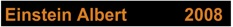
\includegraphics[width=75mm]{Buchruecken}
%\caption[Beschriftung eines Buchrückens.]{Beispiel für die Beschriftung eines
%Buchrückens.}\label{Abb1}
%\end{figure}
%%Tabelle~\ref{Tab1} ist ein Beispiel dafür, wie eine Tabelle aussehen könnte.
%\begin{table}[htbp]
%\centering
%\begin{tabular}{ | c | c | c | }\hline
%{\bf Datum} & {\bf Thema} & {\bf Raum}\\ \hline
%\hline
%20. 08. 2008 & Graphentheorie & HS 3.13\\ \hline
%01. 10. 2008 & Biomathematik & HS 1.05\\ \hline
%\end{tabular}
%\caption[Semesterplan "`Angewandte Mathematik"'.]{Beispiel für einen
%Semesterplan "`Angewandte Mathematik"'.}\label{Tab1}
%\end{table}

%\noindent
%Nun ein Beispiel für eine abgesetzte Formel:
%\begin{equation}
%x =  - \frac{p}{2} \pm \sqrt{\left(\frac{p}{2}\right)^2 - q}.
%\end{equation}
%Und eine mehrzeilige Formel:
%\begin{eqnarray}
%f(t)&=& t^2 \label{For1},\\
%g(t) &=& t-1.
%\end{eqnarray}
%Hier wird auf die Formel (\ref{For1}) verwiesen. \\

%\noindent
%So kann zum Beispiel ein \glqq Source-Code\grqq\  angegeben werden: 
%\begin{verbatim}
%for (i=1; i < 10; i++) {...} 
%\end{verbatim}

%\noindent
%Hier ist ein Hyperlink auf die  \href{http://www.technikum-wien.at}{Homepage}
%der FH Technikum Wien. Email-Adressen können so verlinkt werden:
%\href{mailto:homer.simpson@springfield.com}{\texttt{
%homer.simpson@springfield.com}}\\

%\noindent
%In der Bibliothek der Fachhochschule Technikum Wien gibt es verschiedene
%einführende Bücher zum Thema \glqq \LaTeX \grqq, zum Beispiel \cite{kop05},
%\cite{wil06} oder \cite{mgb+05d} (deutsche Version) bzw. \cite{mgb+04e}
%(englische Version). Empfehlenswerte Skripten für \LaTeX-Einsteiger sind z.B.
%\cite{mj00} und \cite{mj95}. Sie sind frei im Internet verfügbar.



% Literaturverzeichnis
% Das Literaturverzeichnis kann auch nach einem allfälligen Anhang positiioniert werden (siehe "`Leitfaden für Bachelor- und Diplomarbeiten"', Version 2.0, Abschnitt 2.9).

% Möglichkeit 1: Erzeugung des Literaturverzeichnisses mit BibTeX:
% Die Quellen sind in der Datei *.bib (hier Literatur.bib) einzugeben. Danach muss diese Vorlage einmal geTeXt werden, dann BibTeX angewendet werden und 
% anschliessend nochmals zweimal geTeXt werden.
% Im Text erfolgt die Zitierung mit dem Anker-Schlüsselwort, z.B. \cite{kop05}.
\bibliographystyle{IEEEtran}
\bibliography{Literatur}

% Möglichkeit 2: Erzeugung eines Literaturverzeichnisses ohne BibTeX:
%\begin{thebibliography}{99}
%\bibitem[kop05]{kop05}
%H.~Kopka, {\em LaTeX, Band 1: Einführung}, Pearson Studium, München, 3.~Auflage, 2005.
%\bibitem[knu98]{knu98}
%F.~Mittelbach, M.~Goossens, J.~Braams, D.~Carlisle, and Ch. Rowley, {\em The LaTeX Companion}, 
%Addison-Wesley, 2nd edition, 2004.
%\end{thebibliography}

% Abbildungsverzeichnis
\listoffigures
\addcontentsline{toc}{chapter}{Abbildungsverzeichnis} % fügt den Eintrag äbbildungsverzeichnis" im Inhaltsverzeichnis hinzu
\newpage

% Tabellenverzeichnis
%\listoftables 
%\addcontentsline{toc}{chapter}{Tabellenverzeichnis} % fügt den Eintrag
%"Tabellenverzeichnis" im Inhaltsverzeichnis hinzu
%\newpage

% Abkürzungsverzeichnis
% Bei Verwendung der Dokumentklasse "scrartcl" ist der Befehlt \addchap{Abkürzungsverzeichnis} durch 
% \addsec{Abkürzungsverzeichnis} zu ersetzen
\addchap{Abkürzungsverzeichnis}
\hspace{-17mm}\begin{tabular}{>{\raggedleft}p{0.2\linewidth} p{0.75\linewidth} p{0.1\linewidth}}

www & World Wide Web\\
CSS & Cascading Style Sheets\\
AJAX & Asynchron JavaScript And XML\\
HTML & HyperText Markup Language\\
DOM & Document Object Model\\
W3C & World Wide Web Consortium\\

\end{tabular}

% Anhänge
%\begin{appendix}
%\chapter[Erster Anhang]{überschrift des ersten Anhangs}

%Text Text Text Text Text Text Text Text Text Text Text Text Text Text Text Text
%\end{appendix}

\end{document}
